\documentclass[12pt]{article}

\usepackage[spanish]{babel}
\usepackage[utf8]{inputenc}
\usepackage[T1]{fontenc}
\usepackage{amsmath}
\usepackage{graphicx}
\usepackage[top=1.5cm,bottom=2.5cm,left=2.5cm,right=2.5cm]{geometry}

\begin{document}
	
	\section{Problema 13.17}
Un tractocamión entra a una pendiente descendente de 2 por
ciento viajando a 108 km/h y debe bajar su velocidad a 72 km/h en 300 m.
La cabina tiene una masa de 1 800 kg y el remolque de 5 400 kg. Determine
a) la fuerza de frenado promedio que se debe aplicar, b) la fuerza promedio
ejercida sobre el acoplamiento si 70 por ciento de la fuerza de frenado la
proporciona el remolque y 30 por ciento la cabina.
	

	
	\bigskip
	
	\begin{center}
		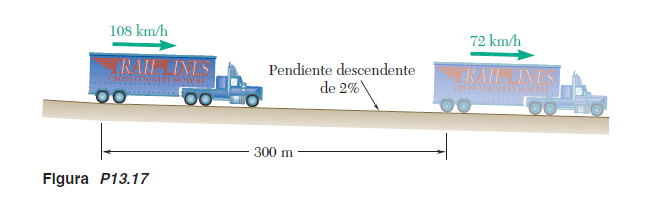
\includegraphics[width=0.8\textwidth]{imagen3}
	\end{center}
	
\end{document}
